\section{Exploratory Data Analysis}

\begin{table}[H]
\centering
\begin{tabular}{|l|l|}
\hline
SN & subject number \\
\hline
treatment & treatment received by each subject ($1$ for intervention and $2$ for control)\\
\hline
month & measurement time (in month)\\
\hline
gender & gender of each subject ($1$ for male and $2$ for female)\\
\hline
education & education received by each subject (in years)\\
\hline
GSI & Global Severity Index: an index indicating level of mental distress\\
\hline
\end{tabular}
\caption{Description of all variables recorded in the study}
\label{tab:var.decription}
\end{table}

\begin{table}[H]
\begin{minipage}{0.5\textwidth}
\centering
\resizebox{\linewidth}{!}{
\begin{tabular}{|l|l|l|l|l|l|l|}
\hline
& education & GSI (0) & GSI (3) & GSI (6) & GSI (18) & GSI (60)\\
\hline
mean & 13.705 & 1.125 & 1.036 & 0.854 & 0.834 & 0.780 \\
\hline
sd & 2.360 & 0.722 & 0.702 & 0.638 & 0.559 & 0.625 \\
\hline
\end{tabular}
}
\caption{Summary statistics for continuous variables}
\label{tab:summ.stat.cont}
\end{minipage}
\hfill
\begin{minipage}{0.5\textwidth}
\centering
\resizebox{\linewidth}{!}{
\begin{tabular}{|l|l|l|l|l|l|l|l|}
\hline
& gender & education & GSI (0) & GSI (3) & GSI (6) & GSI (18) & GSI (60)\\
\hline
count & 4 & 7 & 10 & 38 & 52 & 105 & 98 \\
\hline
proportion & 0.015 & 0.026 & 0.007 & 0.028 & 0.038 & 0.077 & 0.072 \\
\hline
\end{tabular}
}
\caption{Missing rates of all variables in the study}
\label{tab:missing.rate}
\end{minipage}
\end{table}

\subsection{Visualization of GSI}

\begin{figure}[H]
\begin{subfigure}{.5\textwidth}
  \centering
  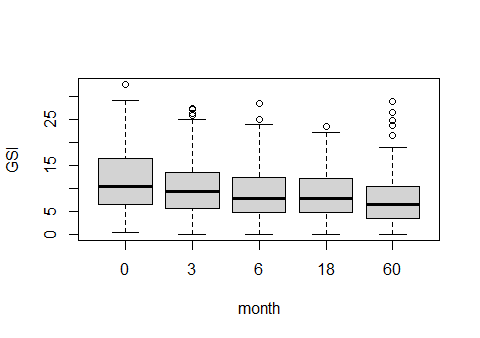
\includegraphics[width=1\linewidth]{../../plots/box_over_time_treatment.png}
  \caption{intervention group (ANOVA: 0, Kruskal-Wallis: 0)}
\end{subfigure}
\hfill
\begin{subfigure}{.5\textwidth}
  \centering
  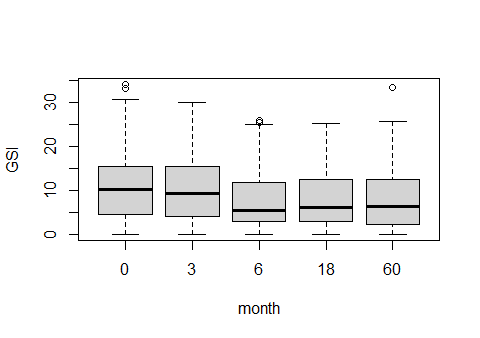
\includegraphics[width=1\linewidth]{../../plots/box_over_time_control.png}
  \caption{control group (ANOVA: 0.021, Kruskal-Wallis: 0.006)}
\end{subfigure}
\caption{Side-by-side boxplots of the GSI scores across measurement times for each treatment group}
\label{fig:boxplot.over.time}
\end{figure}

\begin{figure}[H]
\begin{subfigure}{.19\textwidth}
  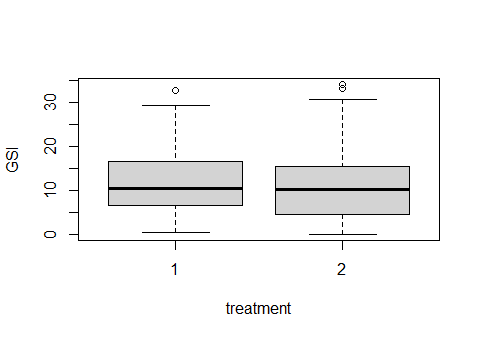
\includegraphics[width=1\linewidth]{../../plots/box_between_group_0.png}
  \caption{baseline (t-test: 0.457, Wilcoxon: 0.271)}
\end{subfigure}
\begin{subfigure}{.19\textwidth}
  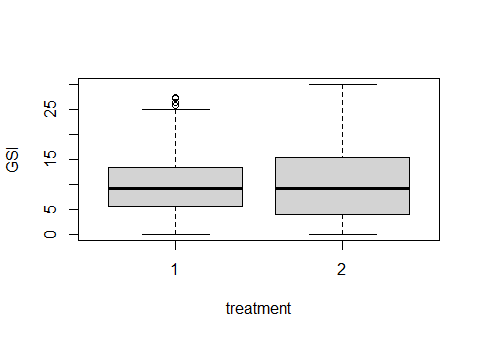
\includegraphics[width=1\linewidth]{../../plots/box_between_group_3.png}
  \caption{3 months (t-test: 0.995, Wilcoxon: 0.489)}
\end{subfigure}
\begin{subfigure}{.19\textwidth}
  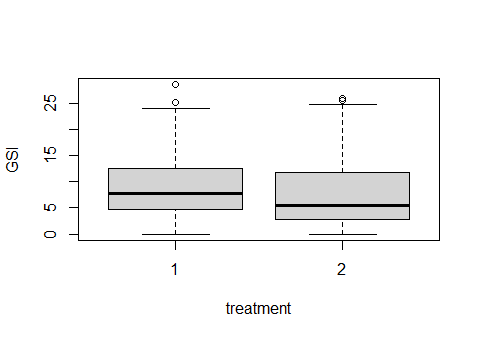
\includegraphics[width=1\linewidth]{../../plots/box_between_group_6.png}
  \caption{6 months (t-test: 0.332, Wilcoxon: 0.084)}
\end{subfigure}
\begin{subfigure}{.19\textwidth}
  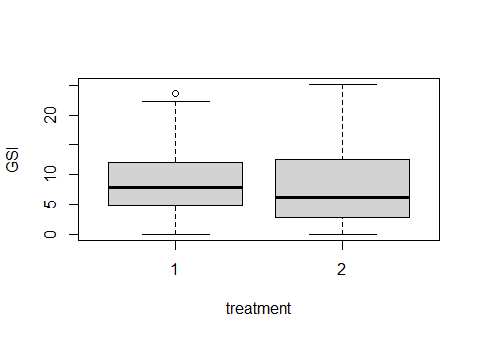
\includegraphics[width=1\linewidth]{../../plots/box_between_group_18.png}
  \caption{18 months (t-test: 0.405, Wilcoxon: 0.167)}
\end{subfigure}
\begin{subfigure}{.19\textwidth}
  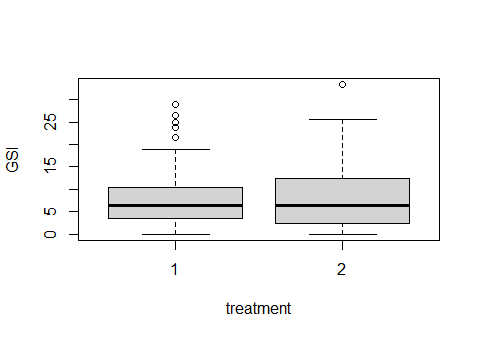
\includegraphics[width=1\linewidth]{../../plots/box_between_group_60.png}
  \caption{60 months (t-test: 0.826, Wilcoxon: 0.831)}
\end{subfigure}
\caption{Side-by-side boxplots of the GSI scores between two treatment groups across measurement times}
\label{fig:boxplot.between.groups}
\end{figure}

\subsection{Correlation between Explanatory Variables}

\begin{figure}[H]
\centering
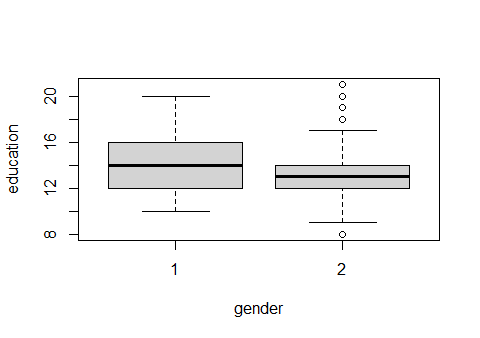
\includegraphics[width=0.5\linewidth]{../../plots/box_correlation.png}
\caption{Side-by-side boxplot of education between the two genders (t-test: 0.014, Wilcoxon: 0.045)}
\label{tab:boxplot.correlation}
\end{figure}

\subsection{Preliminary Conclusions}